% !TEX root = ../thesis.tex
%
\chapter{Results and Evaluation}
\label{sec:evaluation}

\begin{figure}
    \centering
    \begin{subfigure}[t]{.32\textwidth}
        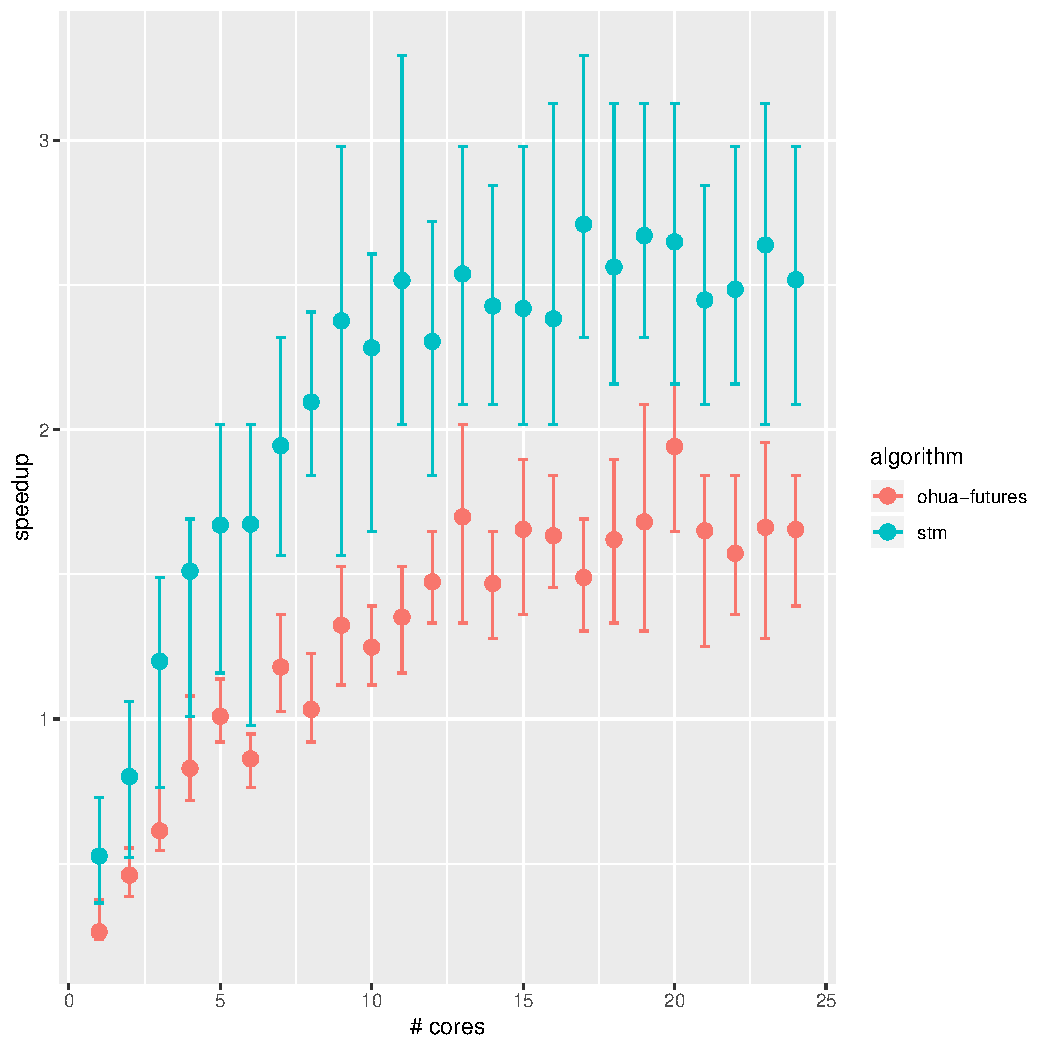
\includegraphics[width=\textwidth,keepaspectratio]{gfx/results/labyrinth/labyrinth}
        \caption{labyrinth}%
    \end{subfigure}%
    ~
    \begin{subfigure}[t]{.32\textwidth}
        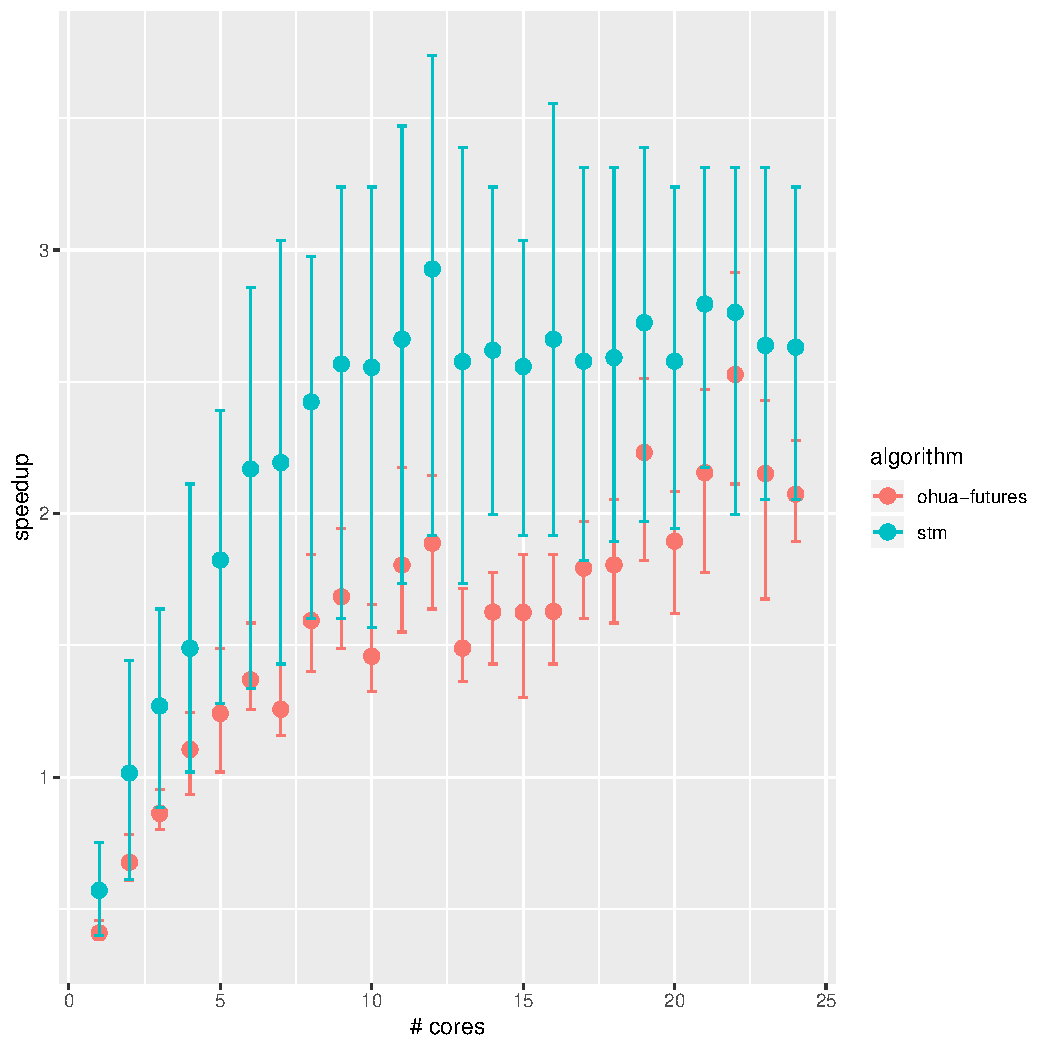
\includegraphics[width=\textwidth,keepaspectratio]{gfx/results/labyrinth/labyrinth+}
        \caption{labyrinth+}%
    \end{subfigure}%
    ~
    \begin{subfigure}[t]{.32\textwidth}
        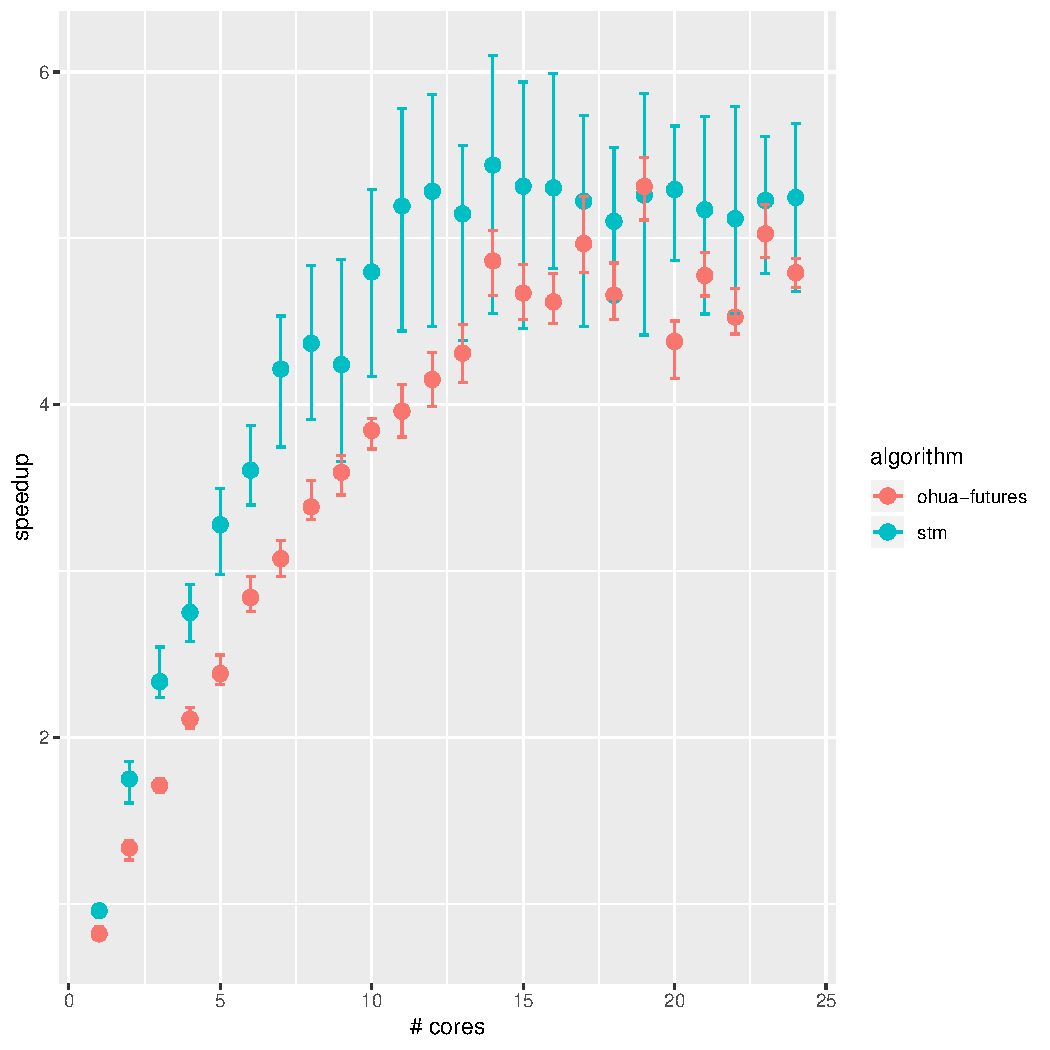
\includegraphics[width=\textwidth,keepaspectratio]{gfx/results/labyrinth/labyrinth++}
        \caption{labyrinth++}%
    \end{subfigure}%

    \begin{subfigure}[t]{.32\textwidth}
        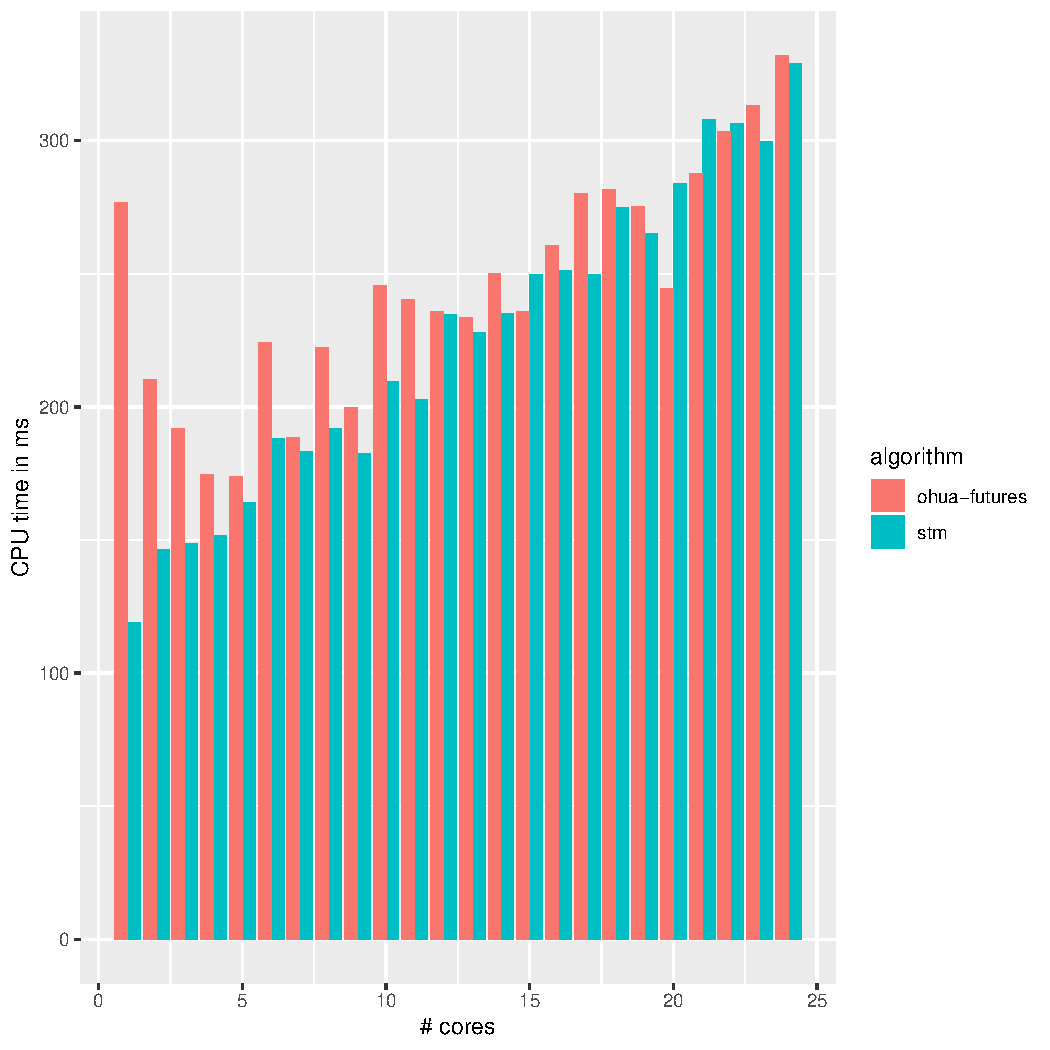
\includegraphics[width=\textwidth,keepaspectratio]{gfx/results/labyrinth/labyrinth_cpu}
        \caption{cpu usage labyrinth}%
    \end{subfigure}%
    ~
    \begin{subfigure}[t]{.32\textwidth}
        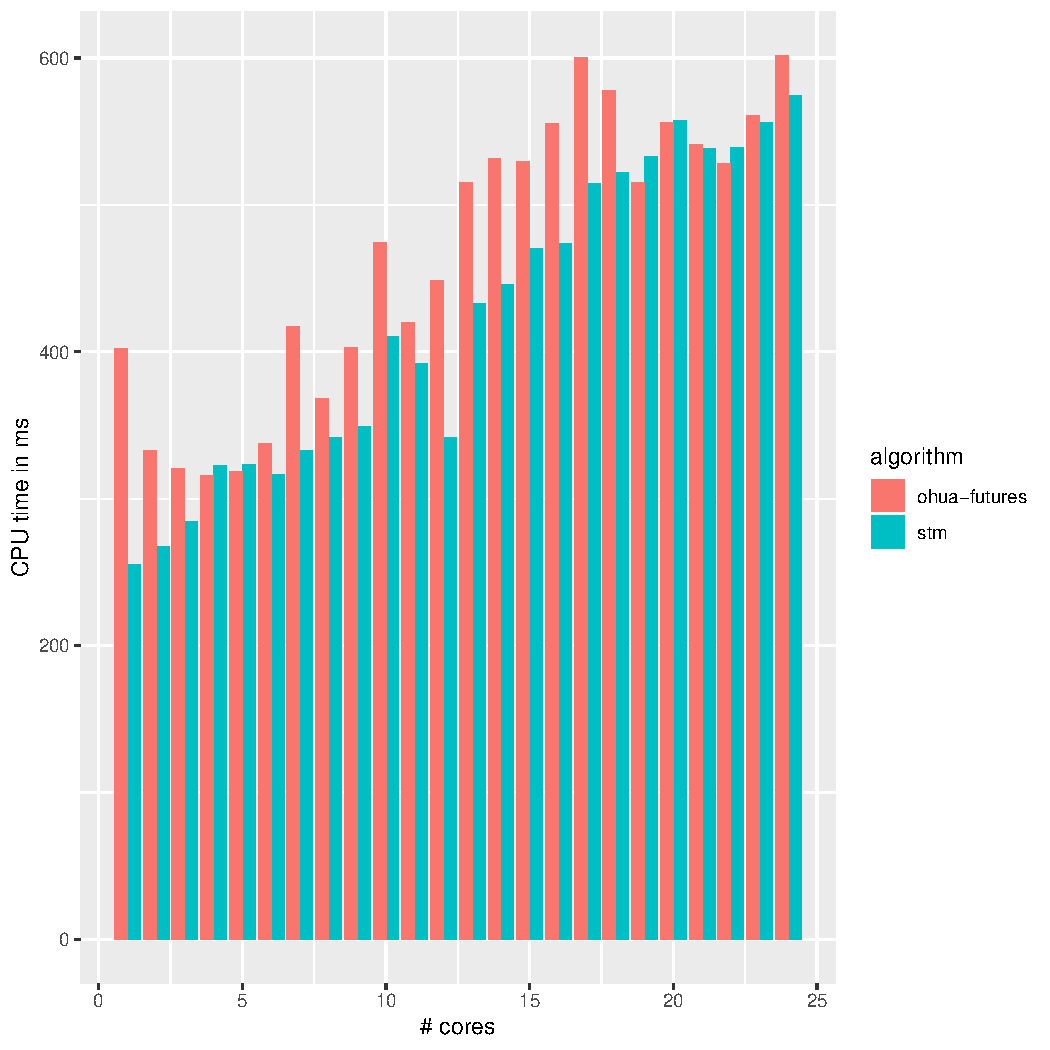
\includegraphics[width=\textwidth,keepaspectratio]{gfx/results/labyrinth/labyrinth+_cpu}
        \caption{cpu usage labyrinth+}%
    \end{subfigure}%
    ~
    \begin{subfigure}[t]{.32\textwidth}
        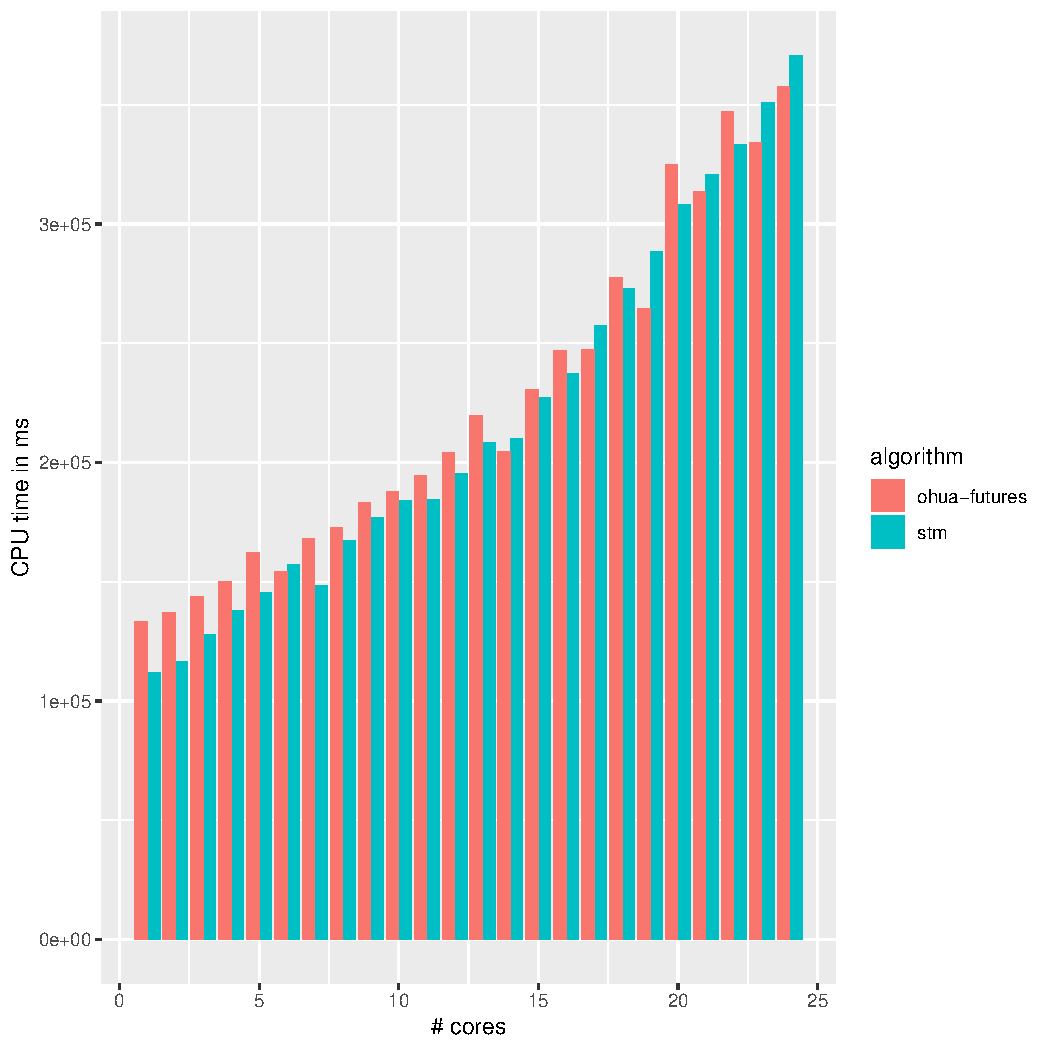
\includegraphics[width=\textwidth,keepaspectratio]{gfx/results/labyrinth/labyrinth++_cpu}
        \caption{cpu usage labyrinth++}%
    \end{subfigure}%
    \caption{Results of the labyrinth benchmark.}%
    \label{fig:evaulation:labyrinth}
\end{figure}

\begin{figure}
    \centering
    \begin{subfigure}[t]{.32\textwidth}
        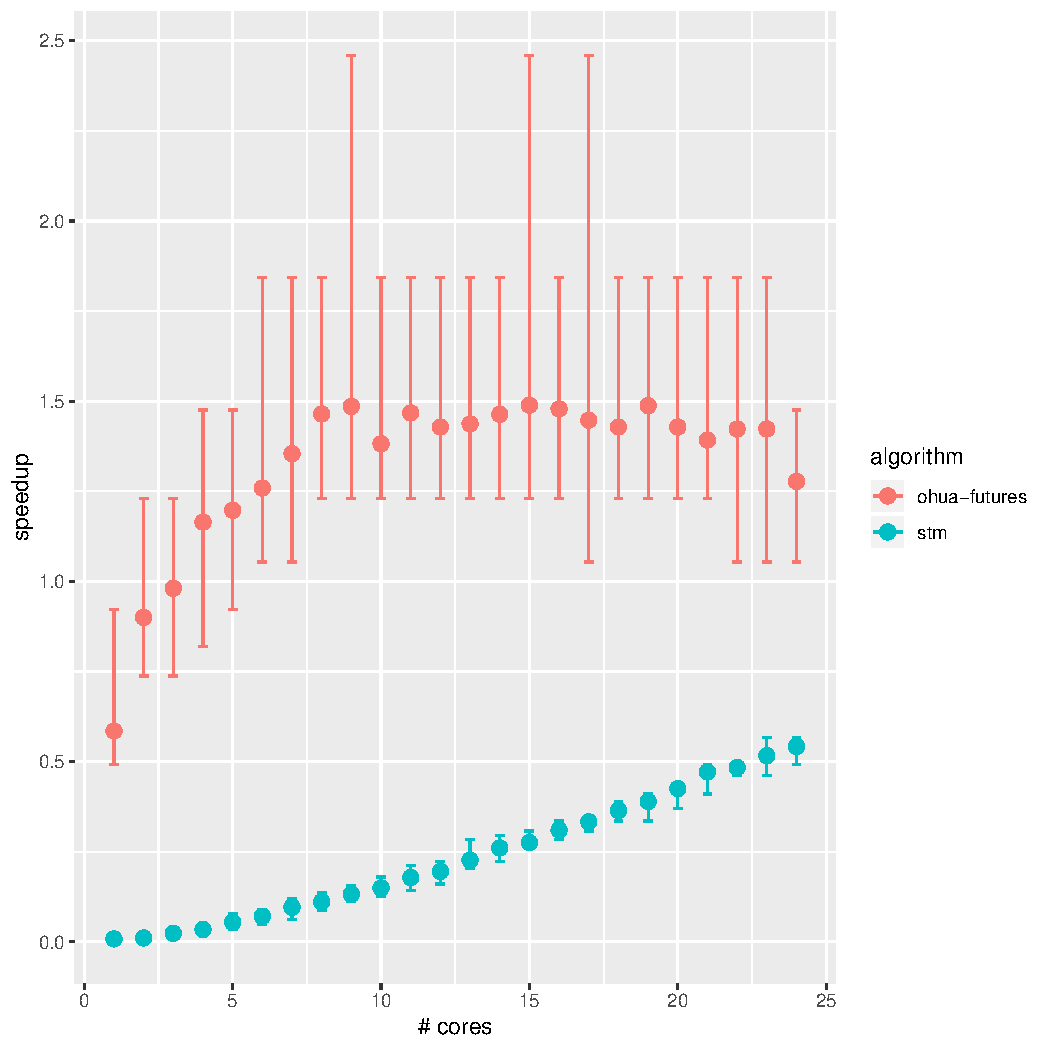
\includegraphics[width=\textwidth,keepaspectratio]{gfx/results/intruder/intruder}
        \caption{intruder}%
    \end{subfigure}%
    ~
    \begin{subfigure}[t]{.32\textwidth}
        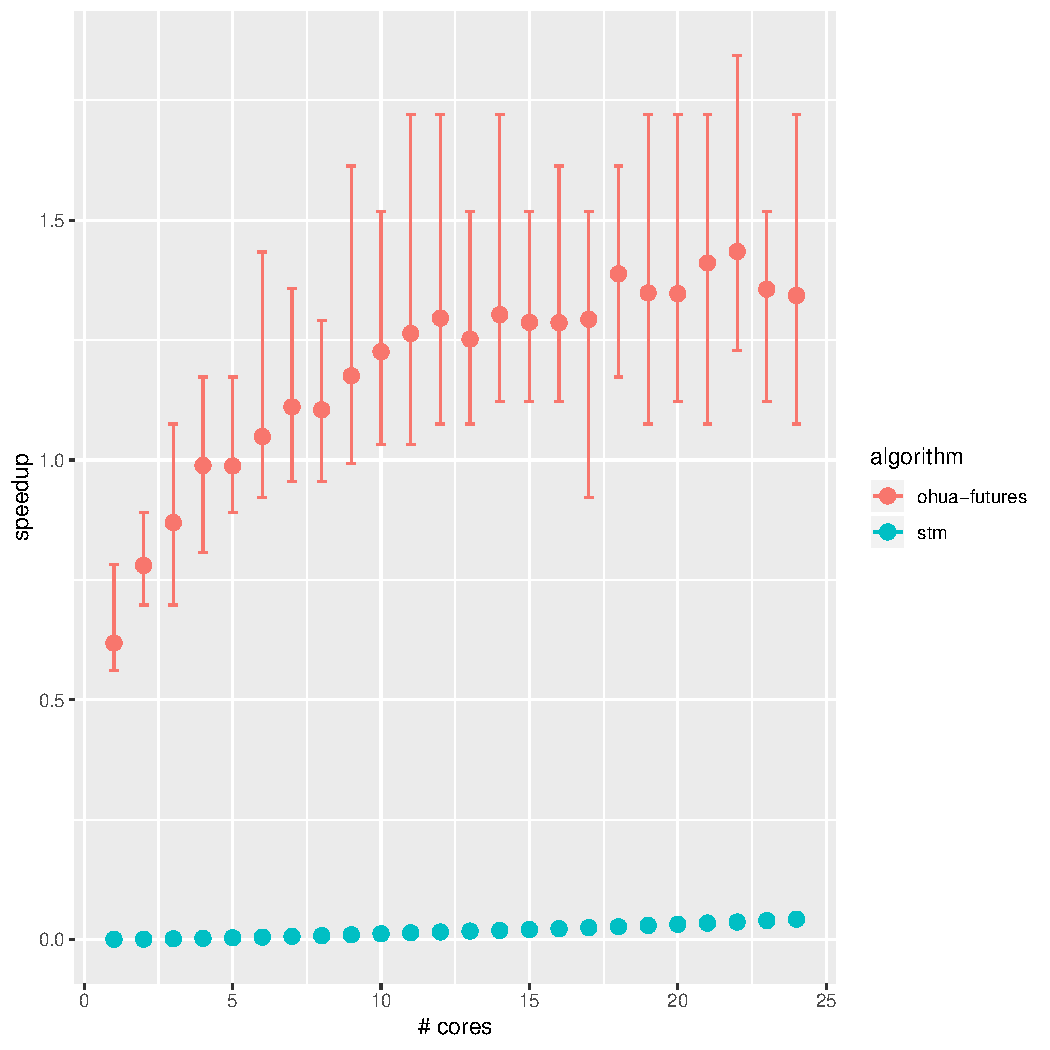
\includegraphics[width=\textwidth,keepaspectratio]{gfx/results/intruder/intruder+}
        \caption{intruder+}%
    \end{subfigure}%
    % ~
    % \begin{subfigure}[t]{.32\textwidth}
    %     \includegraphics[width=\textwidth,keepaspectratio]{gfx/results/intruder/intruder++}
    %     \caption{intruder++}%
    % \end{subfigure}%

    \begin{subfigure}[t]{.32\textwidth}
        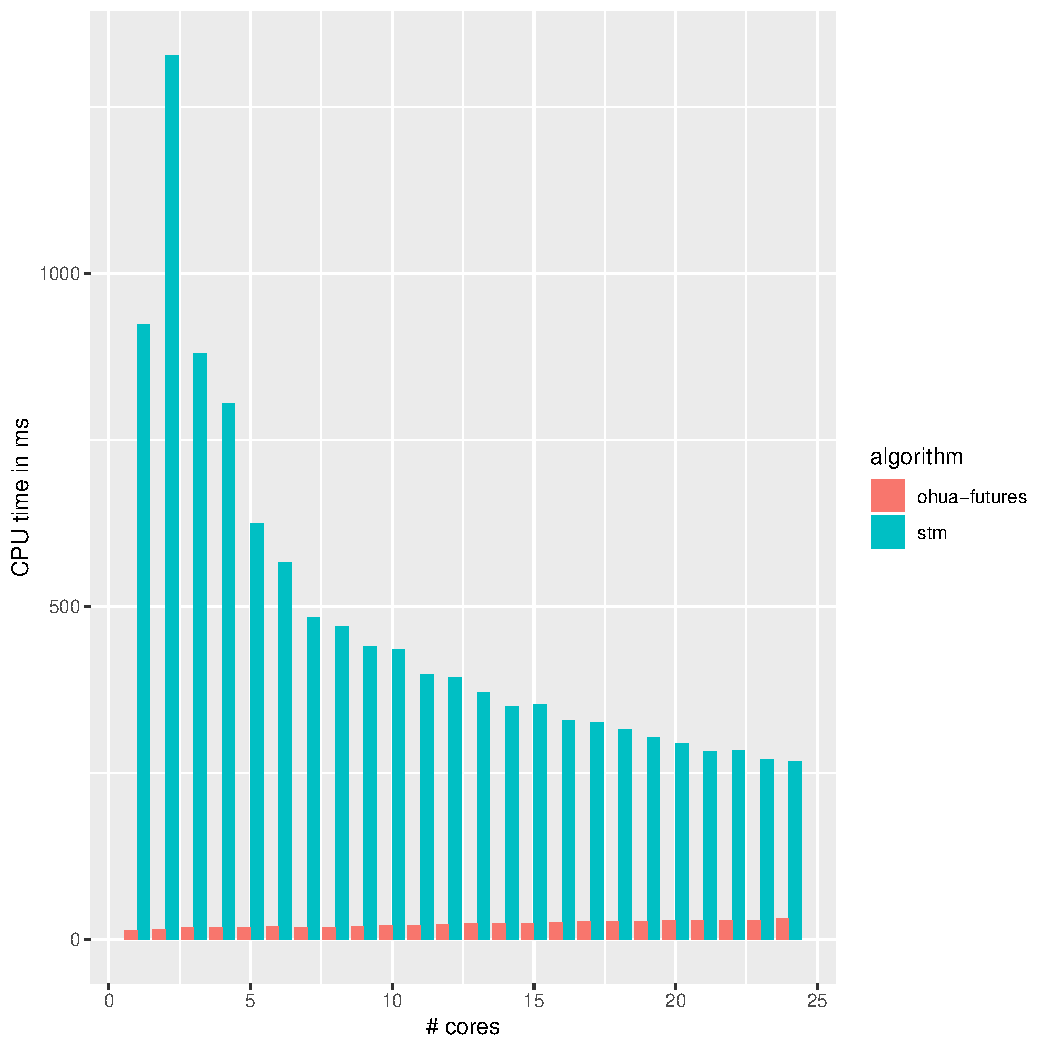
\includegraphics[width=\textwidth,keepaspectratio]{gfx/results/intruder/intruder_cpu}
        \caption{cpu usage intruder}%
    \end{subfigure}%
    ~
    \begin{subfigure}[t]{.32\textwidth}
        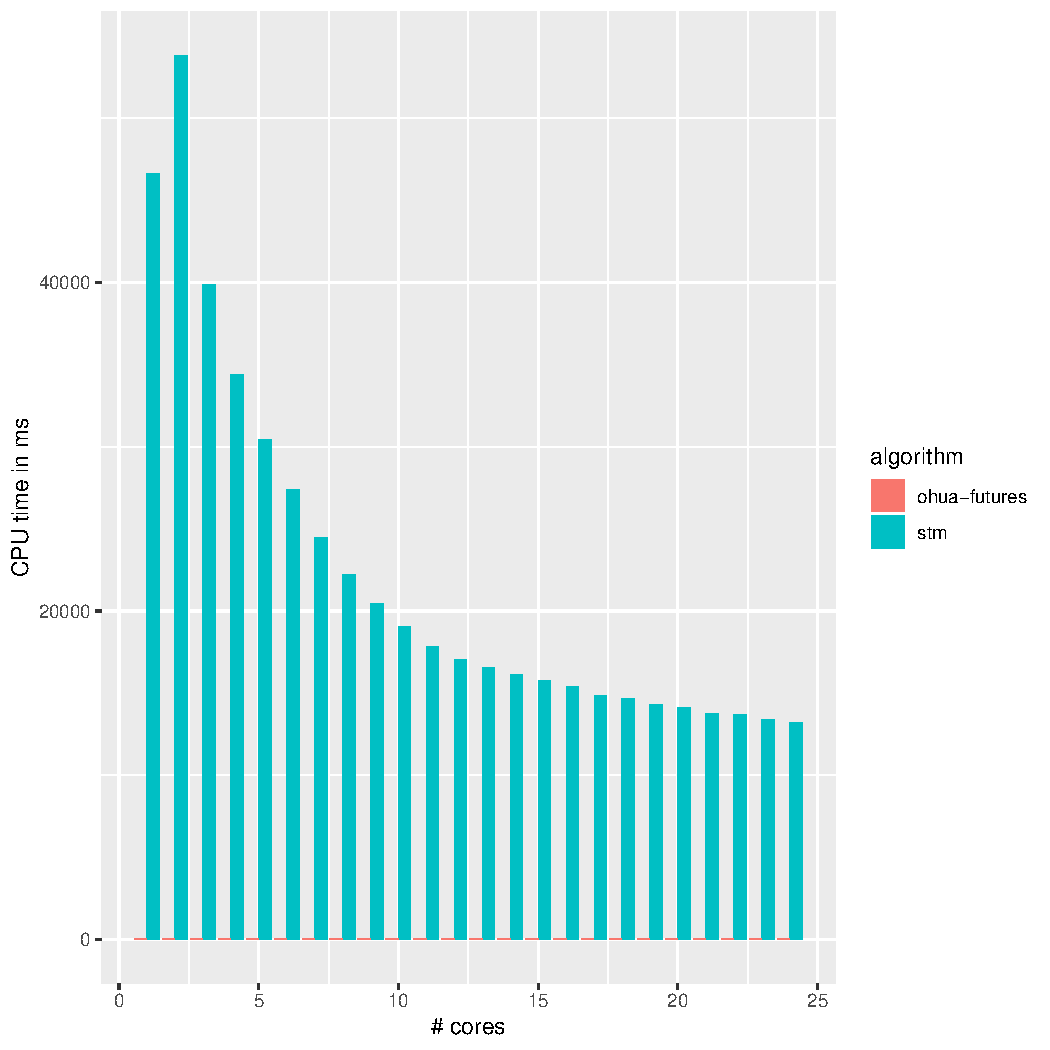
\includegraphics[width=\textwidth,keepaspectratio]{gfx/results/intruder/intruder+_cpu}
        \caption{cpu usage intruder+}%
    \end{subfigure}%
    % ~
    % \begin{subfigure}[t]{.32\textwidth}
    %     \includegraphics[width=\textwidth,keepaspectratio]{gfx/results/intruder/intruder++_cpu}
    %     \caption{cpu usage intruder++}%
    % \end{subfigure}%
    \caption{Results of the intruder benchmark.}%
    \label{fig:evaulation:intruder}
\end{figure}

\begin{figure}
    \centering
    \begin{subfigure}[t]{.32\textwidth}
        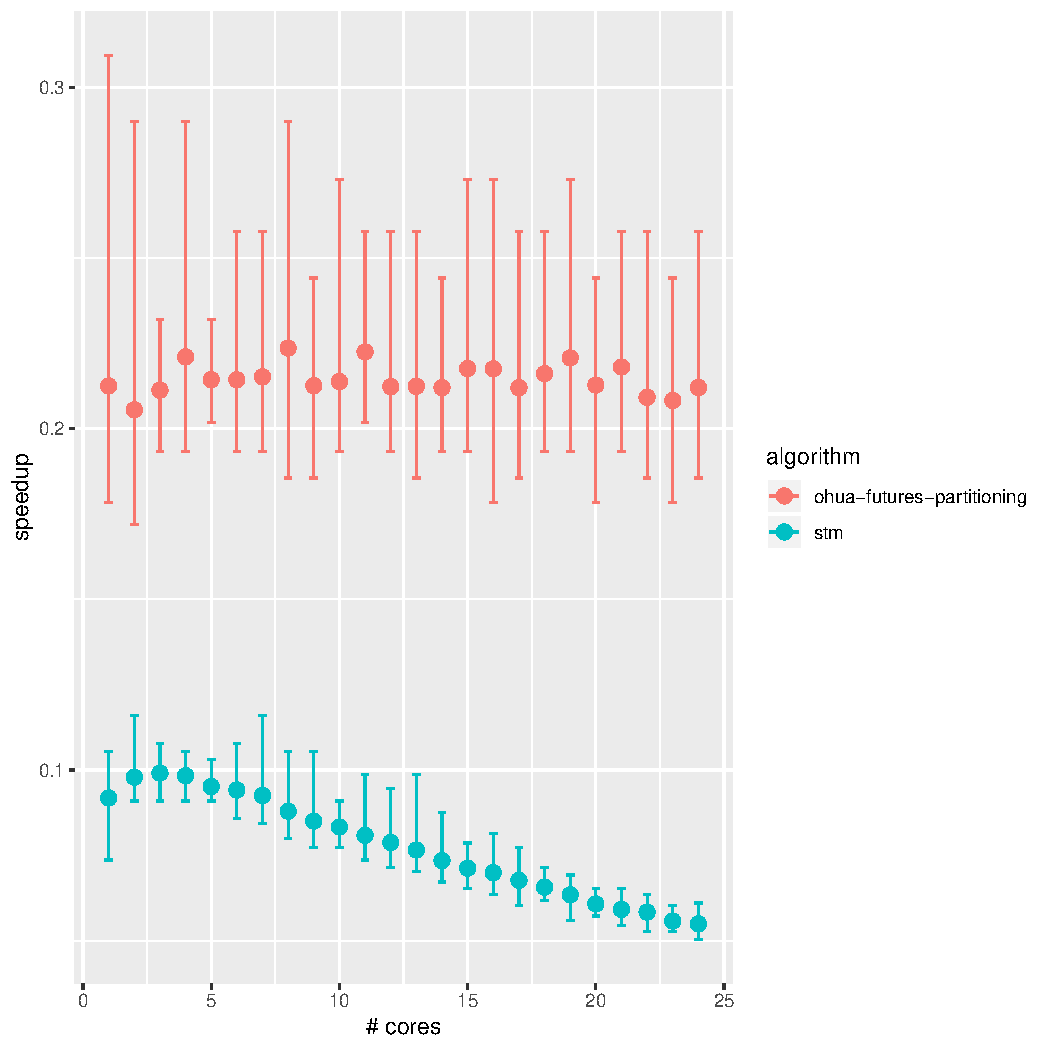
\includegraphics[width=\textwidth,keepaspectratio]{gfx/results/genome/genome}
        \caption{genome}%
    \end{subfigure}%
    ~
    \begin{subfigure}[t]{.32\textwidth}
        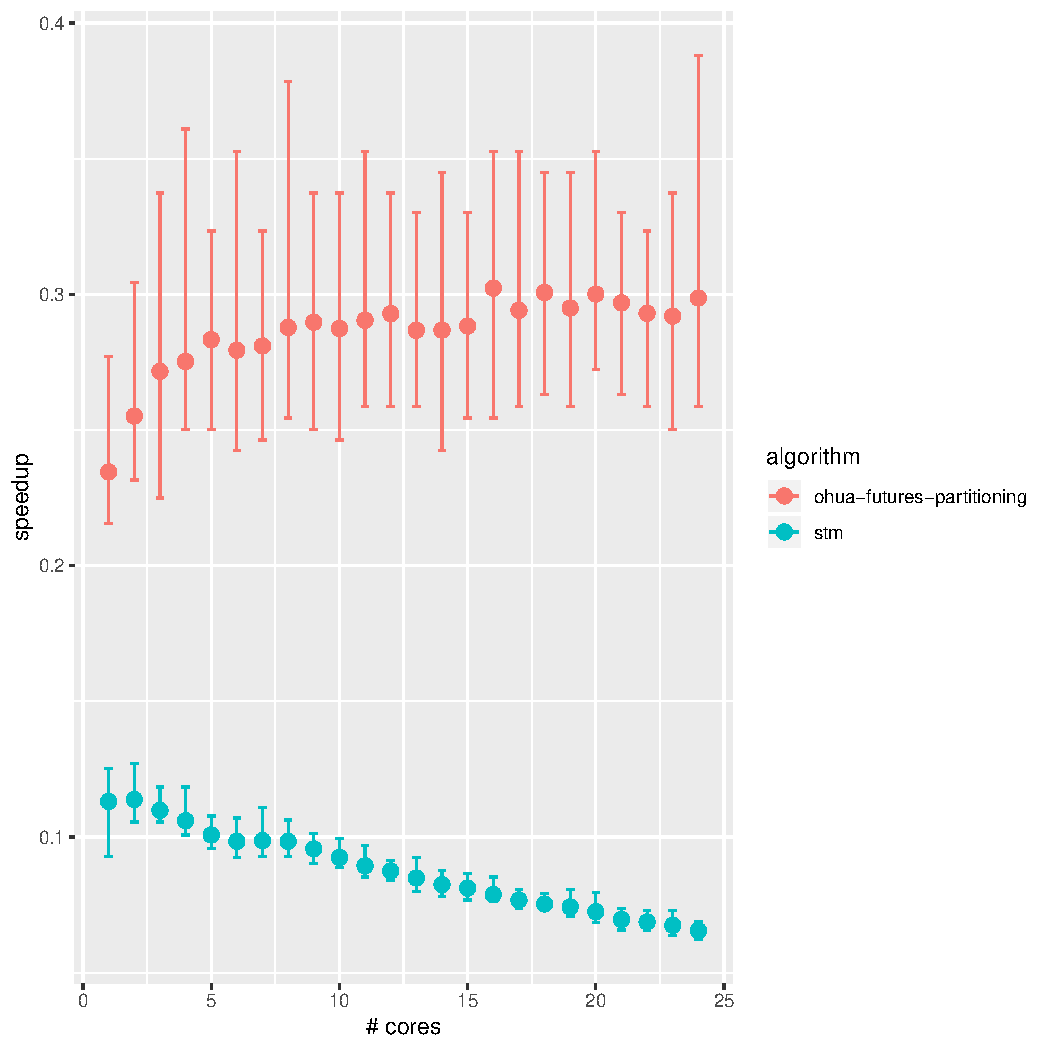
\includegraphics[width=\textwidth,keepaspectratio]{gfx/results/genome/genome+}
        \caption{genome+}%
    \end{subfigure}%
    ~
    \begin{subfigure}[t]{.32\textwidth}
        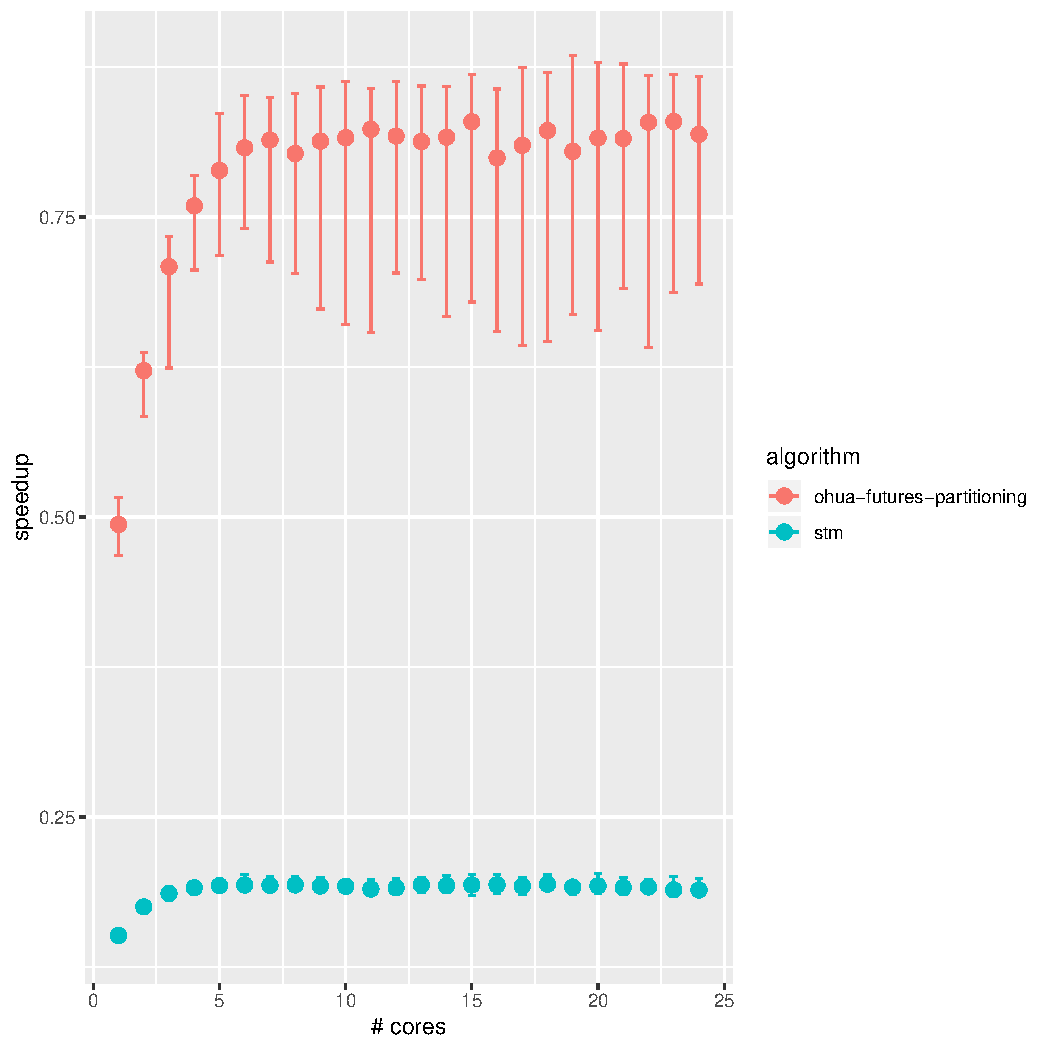
\includegraphics[width=\textwidth,keepaspectratio]{gfx/results/genome/genome++}
        \caption{genome++}%
    \end{subfigure}%

    \begin{subfigure}[t]{.32\textwidth}
        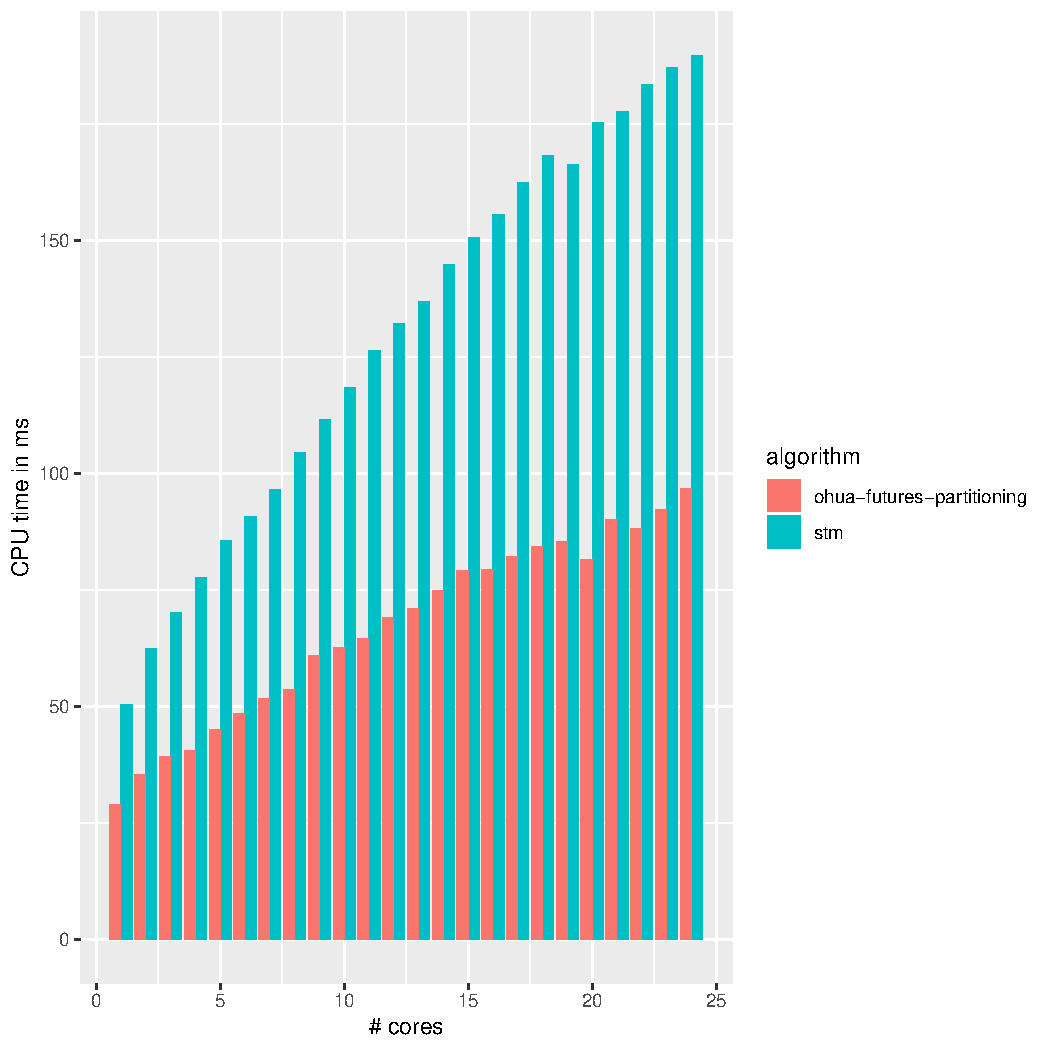
\includegraphics[width=\textwidth,keepaspectratio]{gfx/results/genome/genome_cpu}
        \caption{cpu usage genome}%
    \end{subfigure}%
    ~
    \begin{subfigure}[t]{.32\textwidth}
        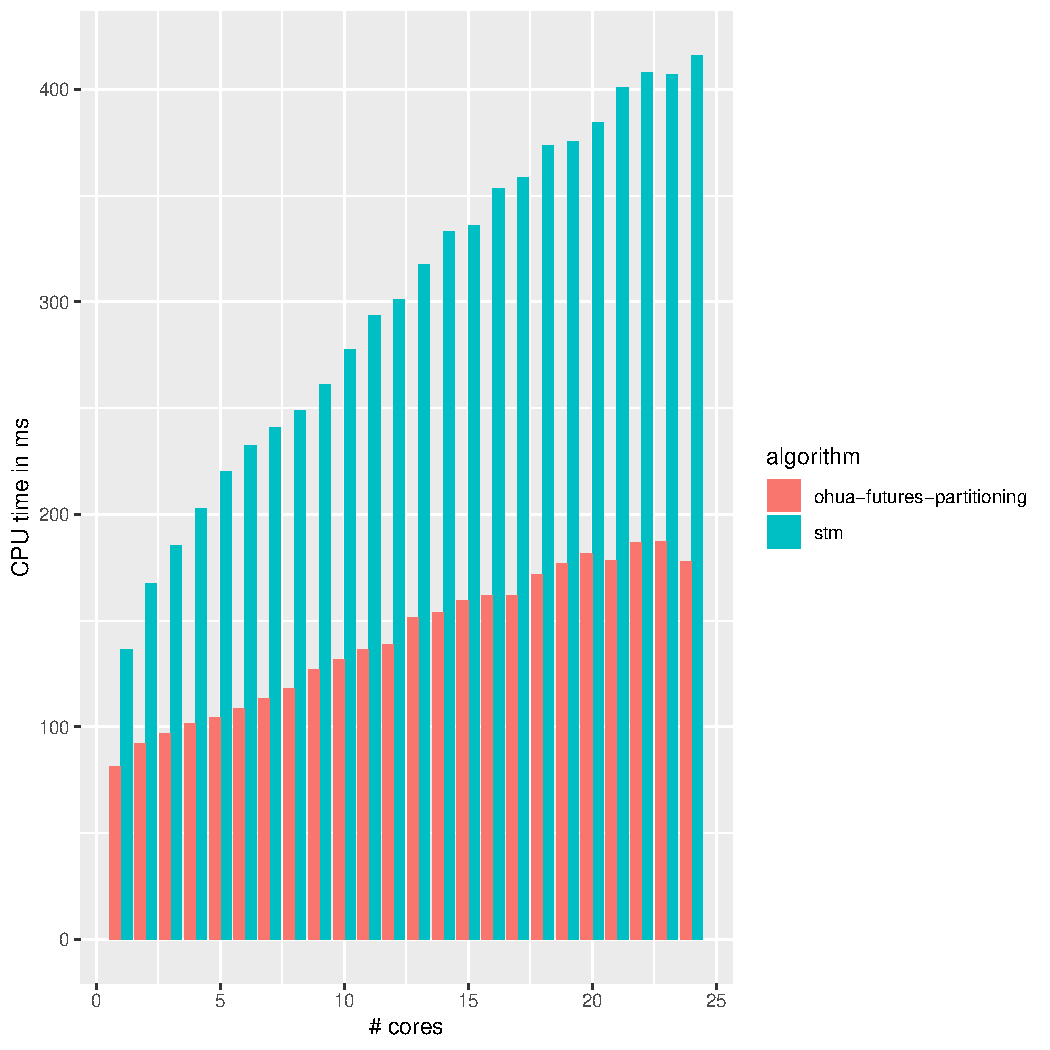
\includegraphics[width=\textwidth,keepaspectratio]{gfx/results/genome/genome+_cpu}
        \caption{cpu usage genome+}%
    \end{subfigure}%
    ~
    \begin{subfigure}[t]{.32\textwidth}
        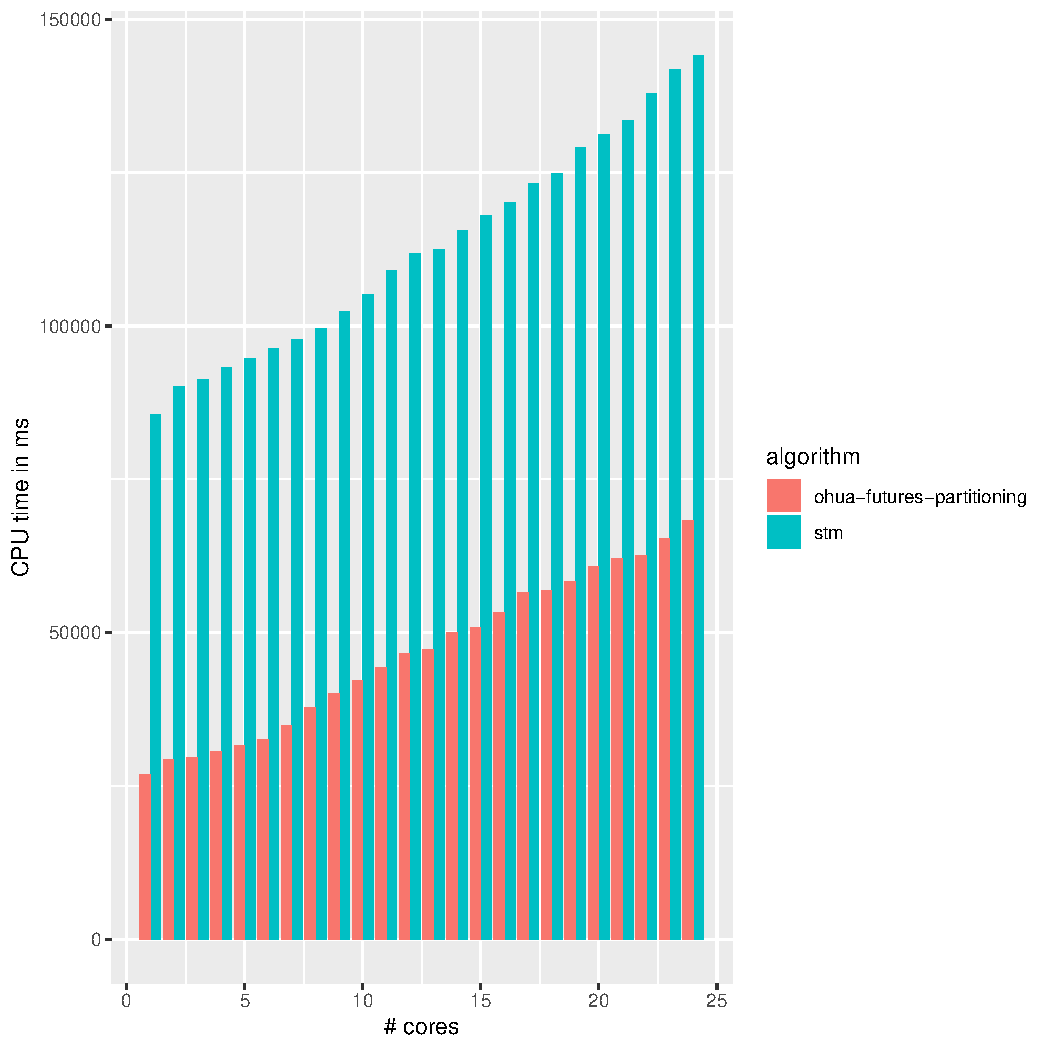
\includegraphics[width=\textwidth,keepaspectratio]{gfx/results/genome/genome++_cpu}
        \caption{cpu usage genome++}%
    \end{subfigure}%
    \caption{Results of the genome benchmark.}%
    \label{fig:evaulation:genome}
\end{figure}

\begin{figure}
    \begin{subfigure}[t]{.32\textwidth}
        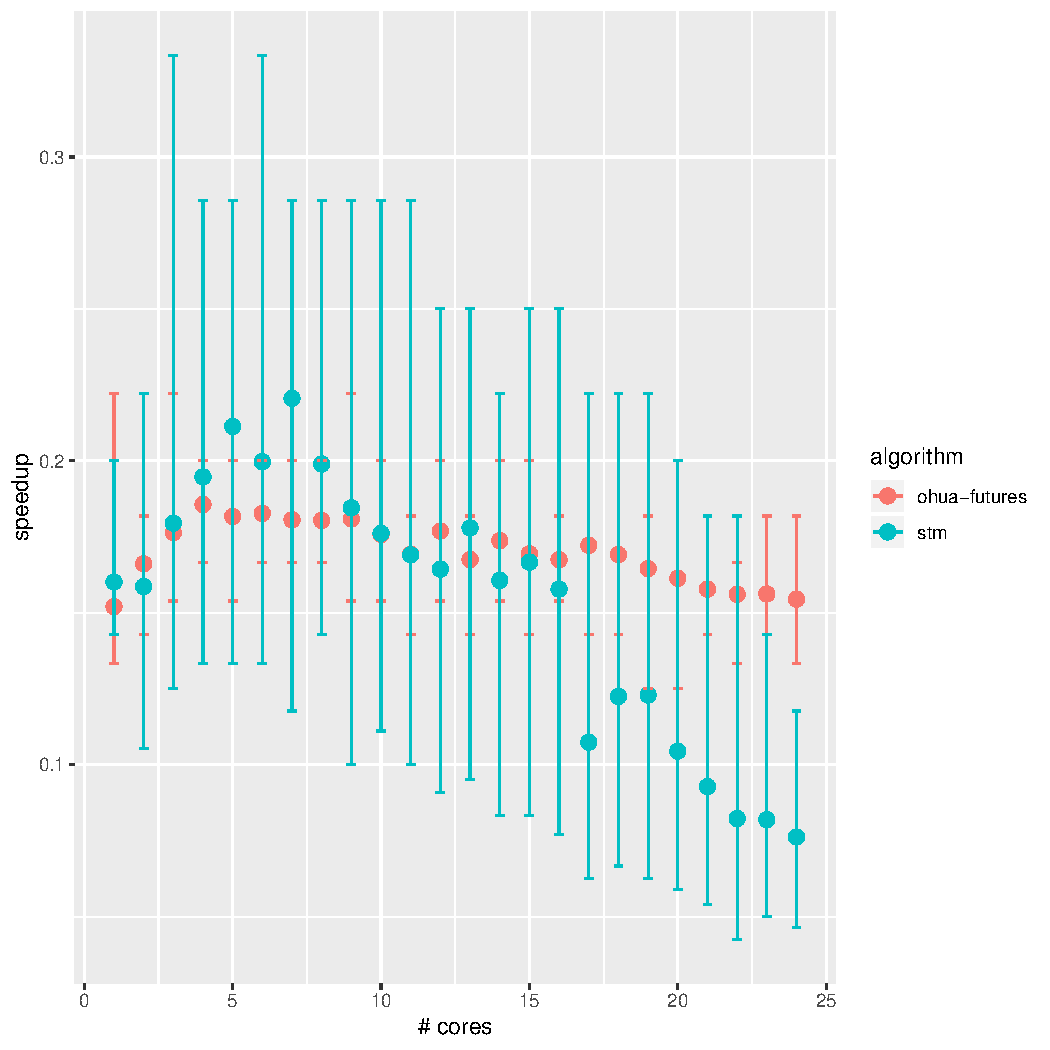
\includegraphics[width=\textwidth,keepaspectratio]{gfx/results/kmeans/kmeans-high}
        \caption{kmeans-high}%
    \end{subfigure}%
    ~
    \begin{subfigure}[t]{.32\textwidth}
        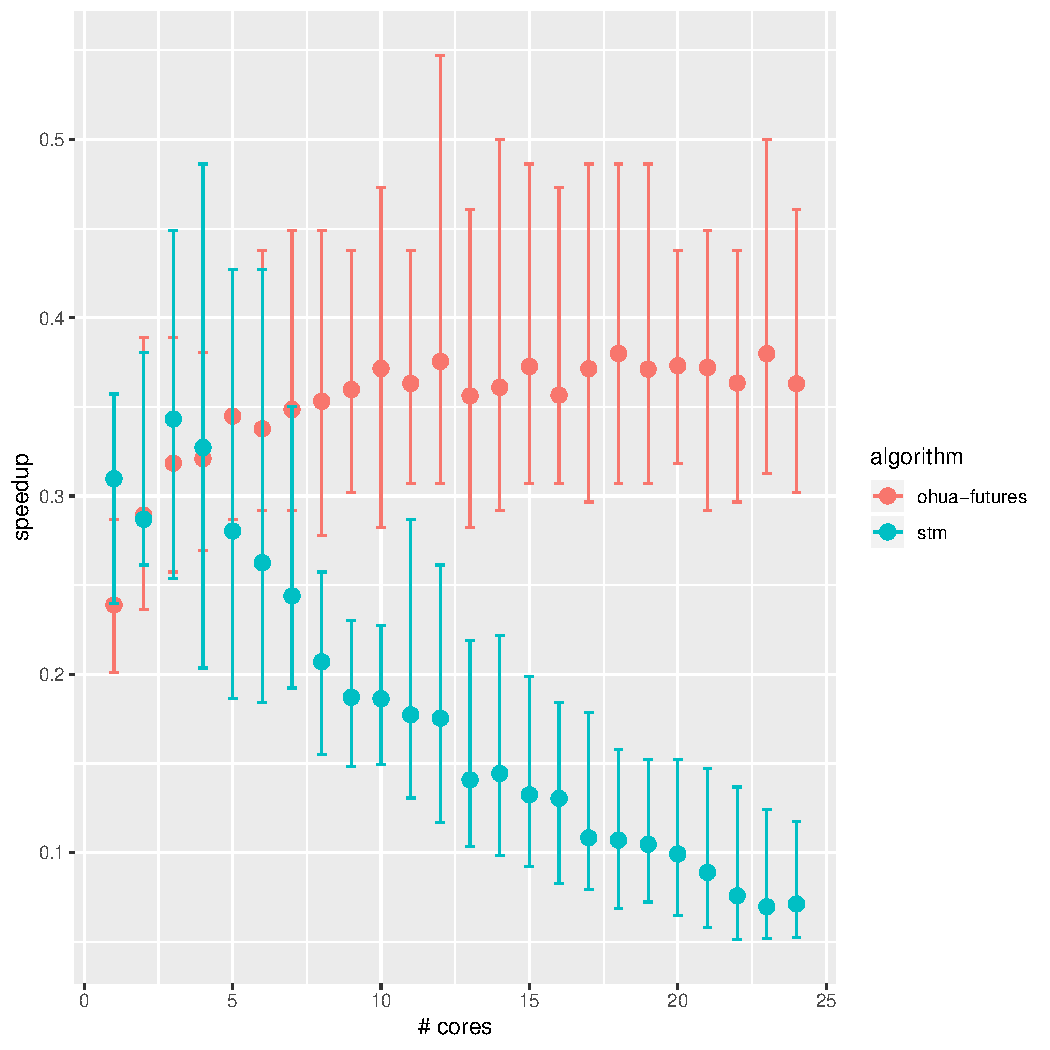
\includegraphics[width=\textwidth,keepaspectratio]{gfx/results/kmeans/kmeans-high+}
        \caption{kmeans-high+}%
    \end{subfigure}%
    ~
    \begin{subfigure}[t]{.32\textwidth}
        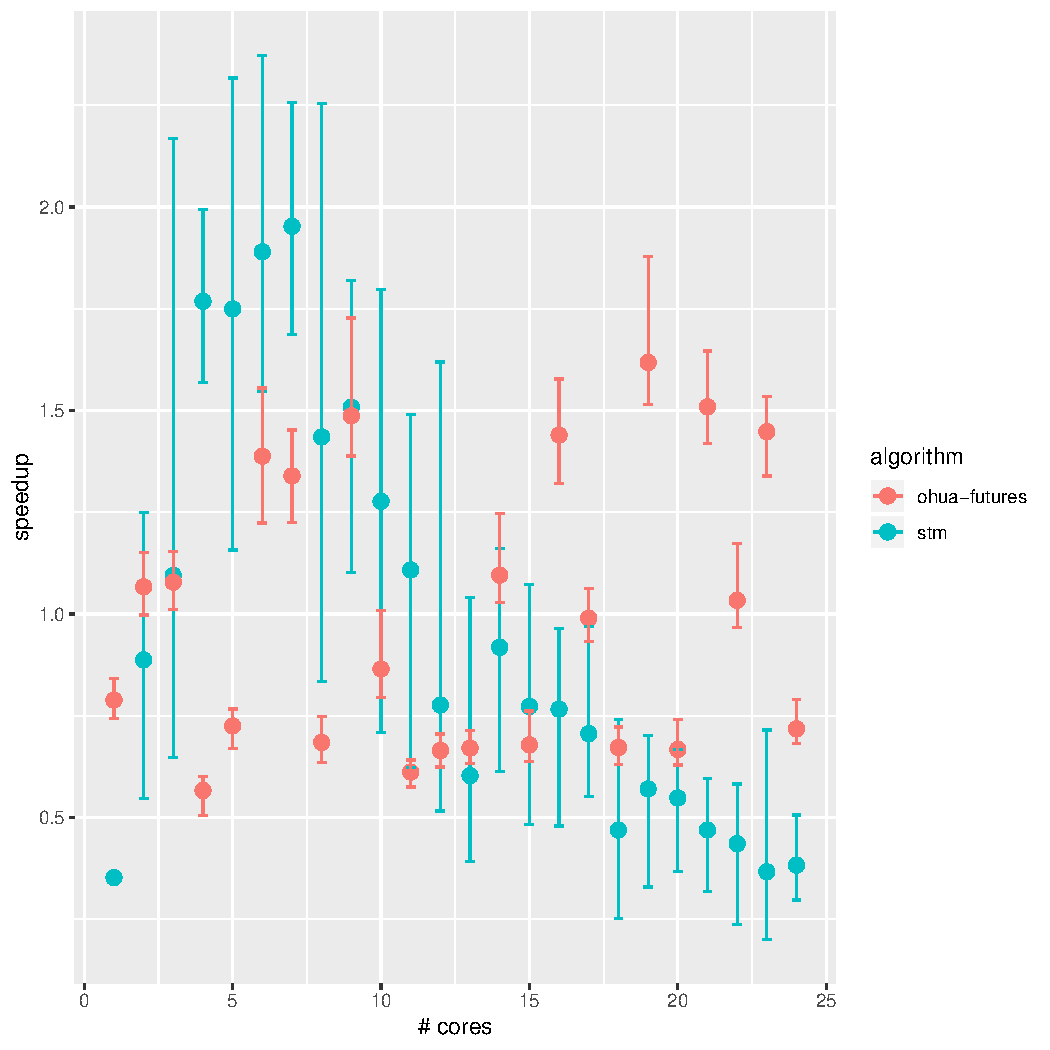
\includegraphics[width=\textwidth,keepaspectratio]{gfx/results/kmeans/kmeans-high++}
        \caption{kmeans-high++}%
    \end{subfigure}%

    \begin{subfigure}[t]{.32\textwidth}
        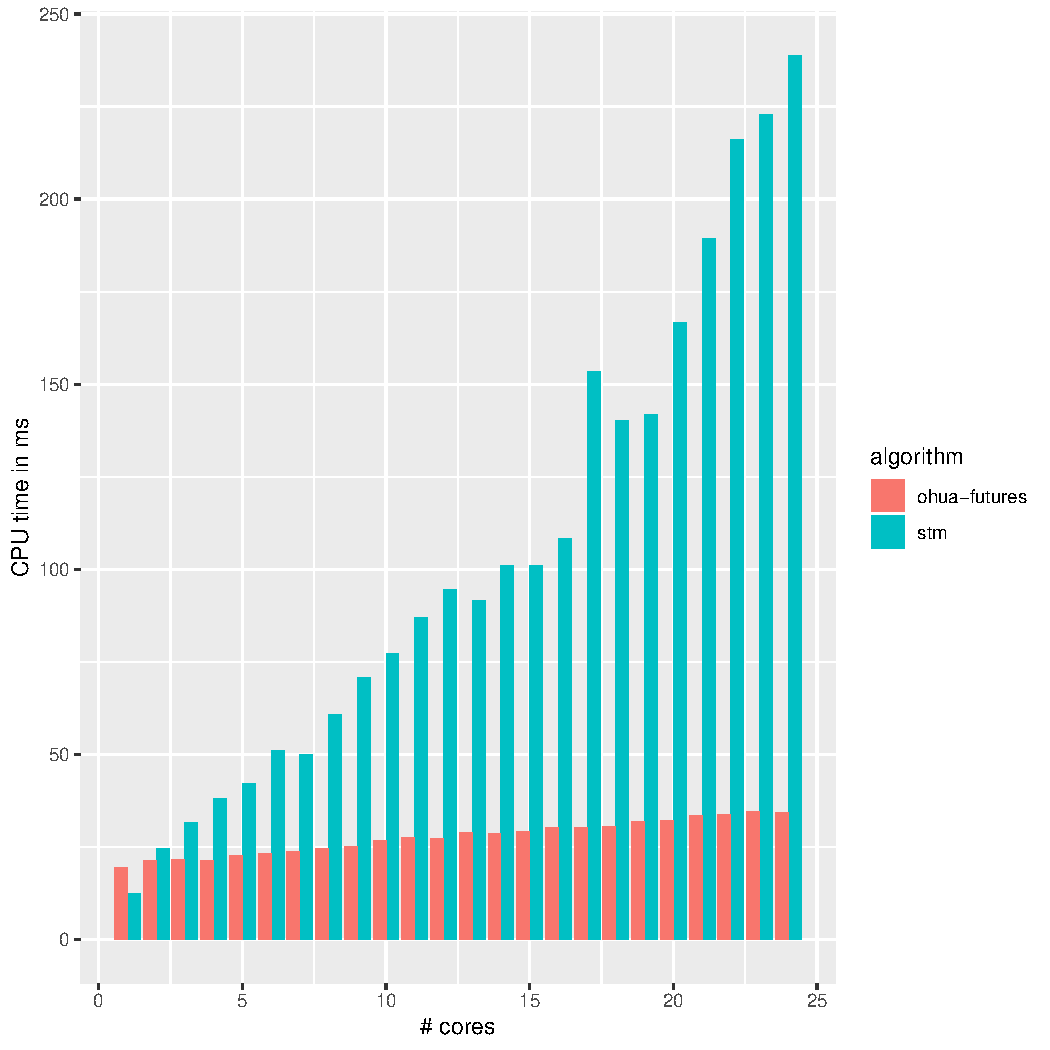
\includegraphics[width=\textwidth,keepaspectratio]{gfx/results/kmeans/kmeans-high_cpu}
        \caption{cpu usage kmeans-high}%
    \end{subfigure}%
    ~
    \begin{subfigure}[t]{.32\textwidth}
        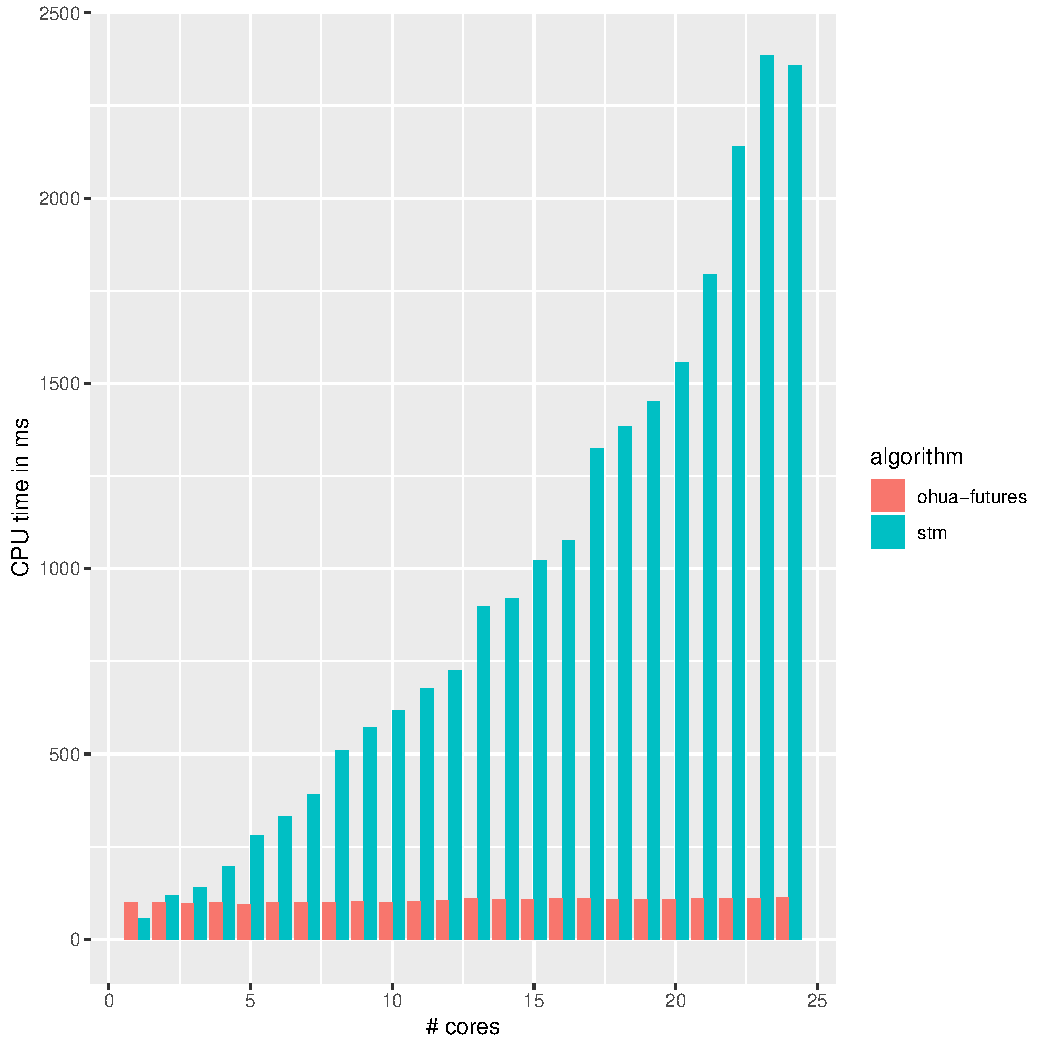
\includegraphics[width=\textwidth,keepaspectratio]{gfx/results/kmeans/kmeans-high+_cpu}
        \caption{cpu usage kmeans-high+}%
    \end{subfigure}%
    ~
    \begin{subfigure}[t]{.32\textwidth}
        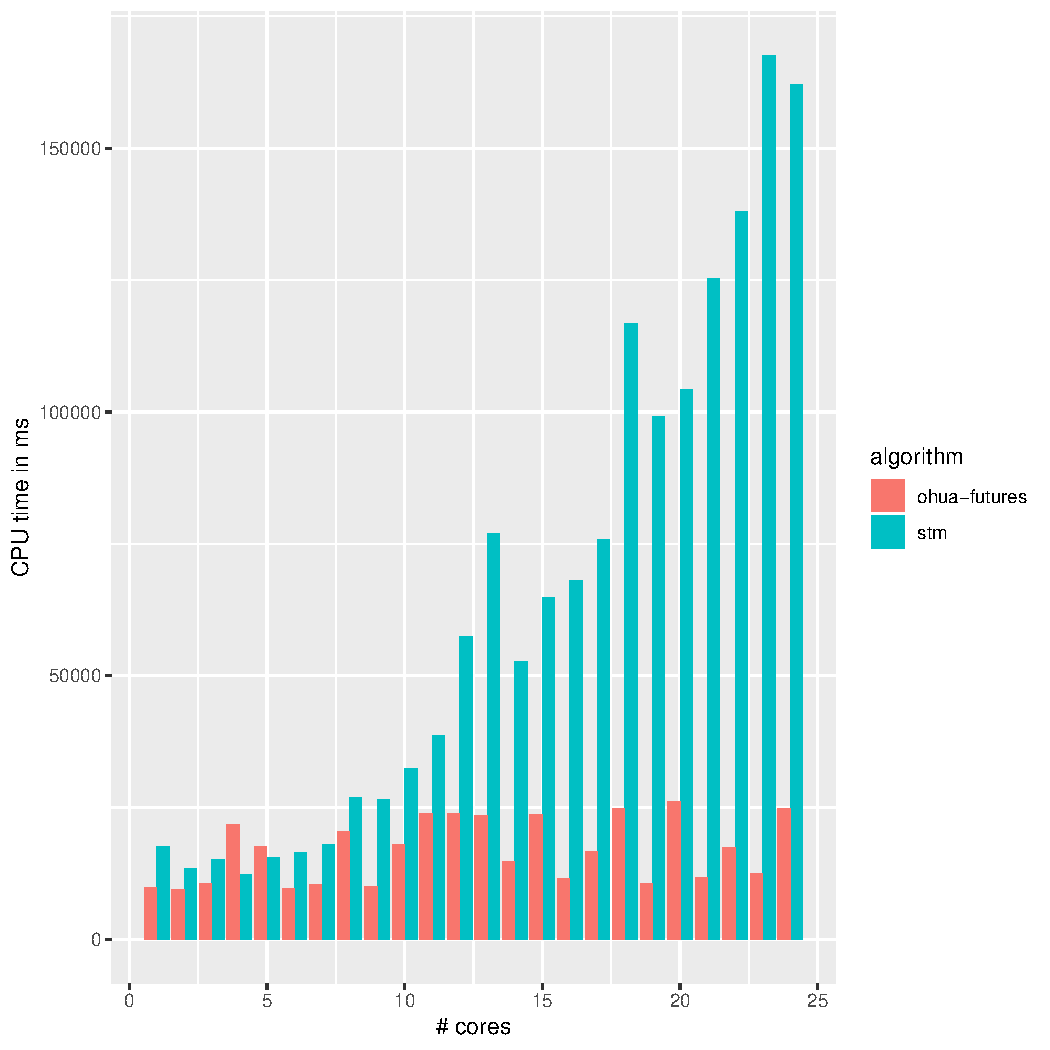
\includegraphics[width=\textwidth,keepaspectratio]{gfx/results/kmeans/kmeans-high++_cpu}
        \caption{cpu usage kmeans-high++}%
    \end{subfigure}%
    \caption{Results of the kmeans-high benchmark.}%
    \label{fig:evaulation:kmeans-high}
\end{figure}

\begin{figure}
    \begin{subfigure}[t]{.32\textwidth}
        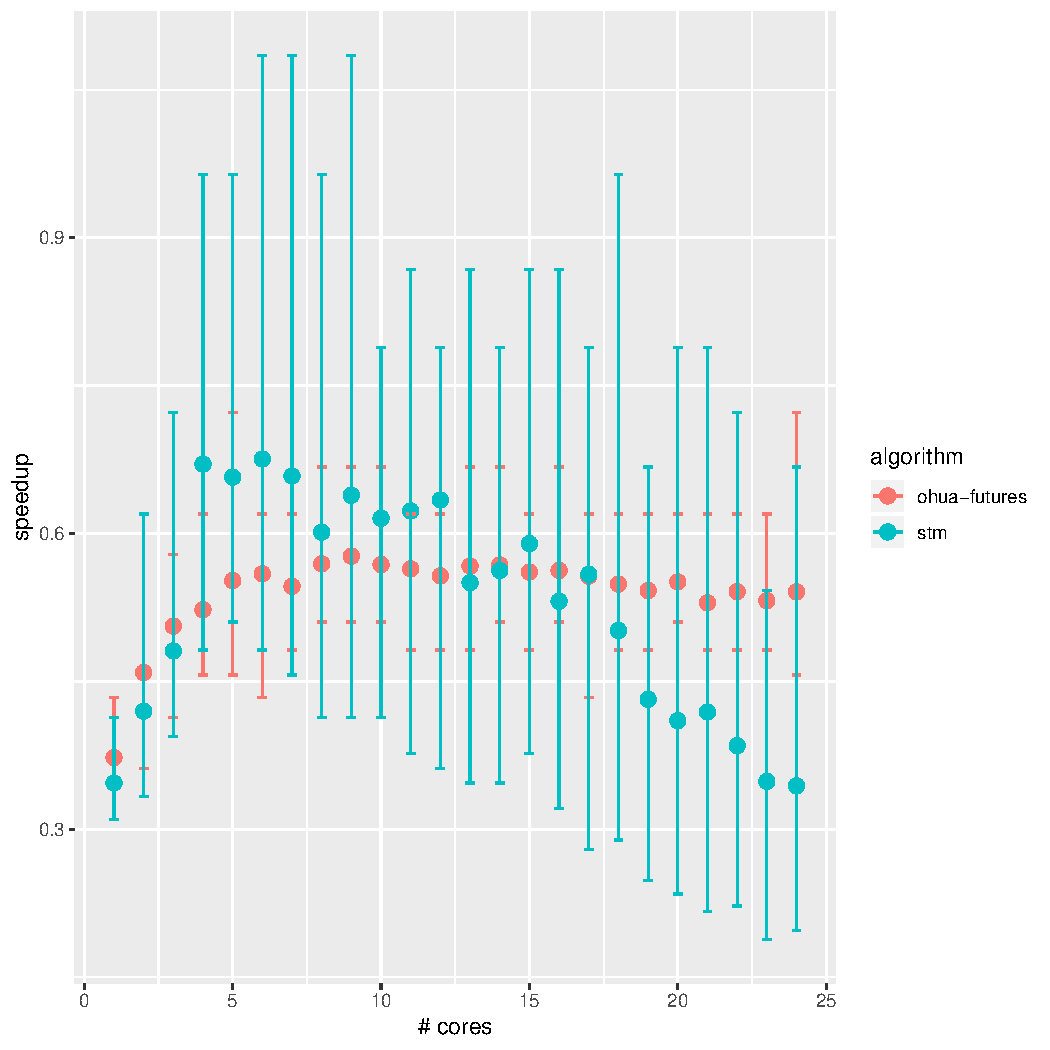
\includegraphics[width=\textwidth,keepaspectratio]{gfx/results/kmeans/kmeans-low}
        \caption{kmeans-low}%
    \end{subfigure}%
    ~
    \begin{subfigure}[t]{.32\textwidth}
        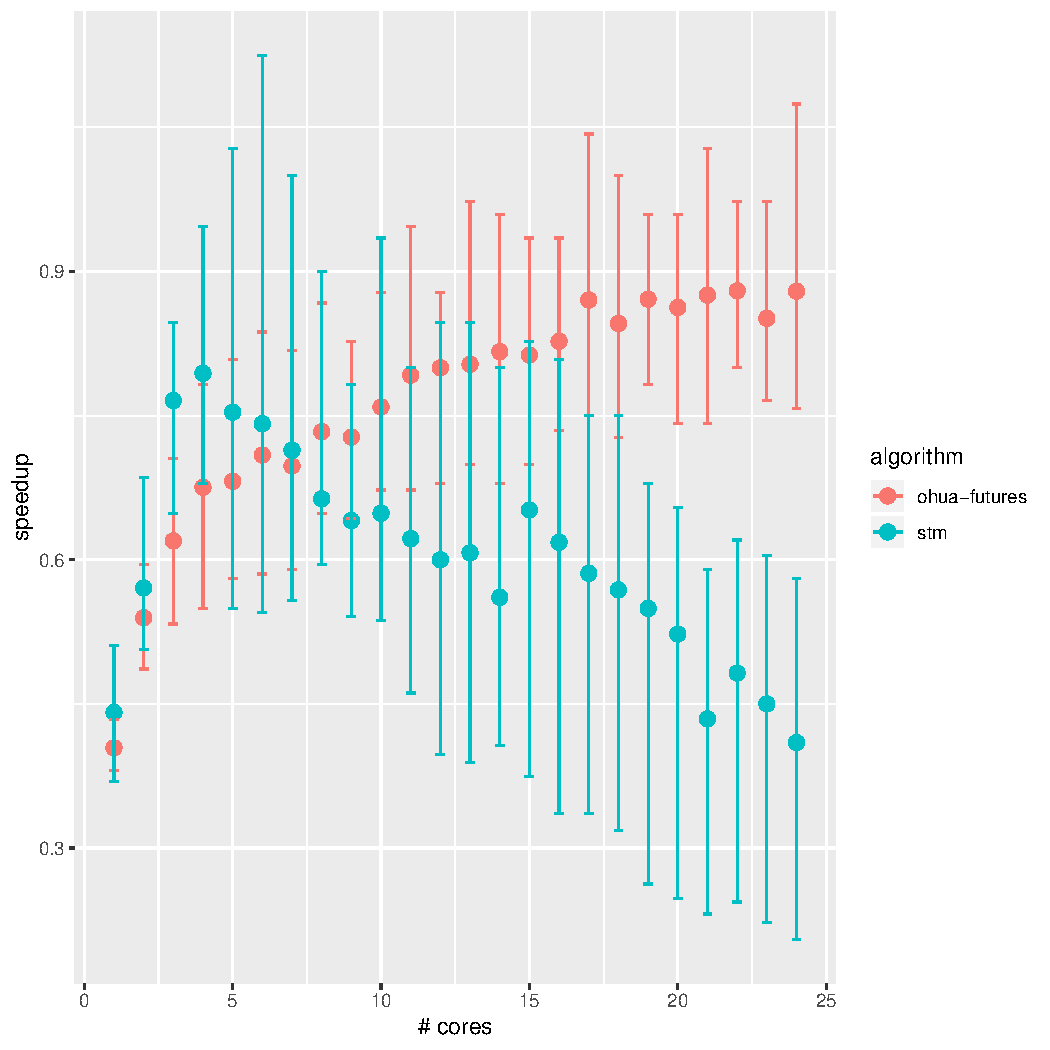
\includegraphics[width=\textwidth,keepaspectratio]{gfx/results/kmeans/kmeans-low+}
        \caption{kmeans-low+}%
    \end{subfigure}%
    ~
    \begin{subfigure}[t]{.32\textwidth}
        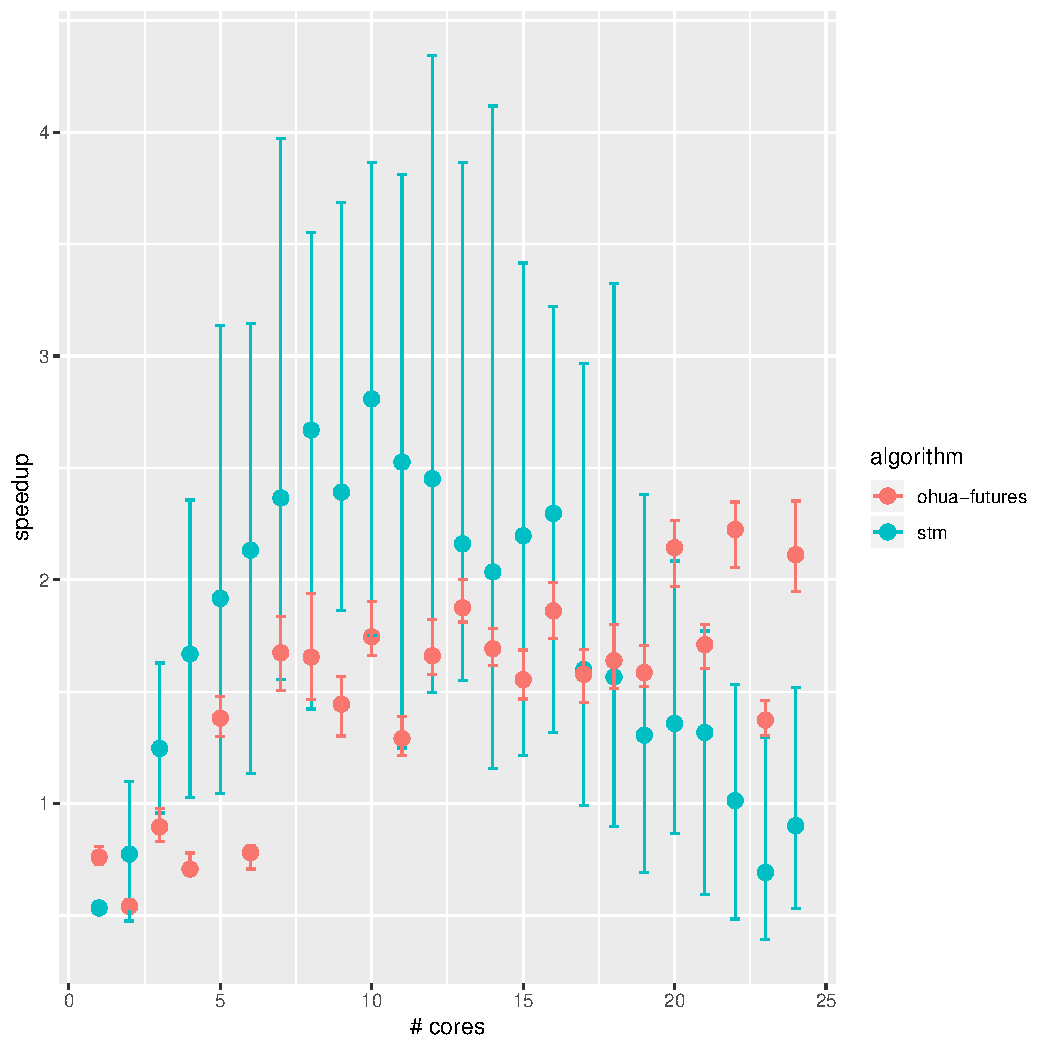
\includegraphics[width=\textwidth,keepaspectratio]{gfx/results/kmeans/kmeans-low++}
        \caption{kmeans-low++}%
    \end{subfigure}%

    \begin{subfigure}[t]{.32\textwidth}
        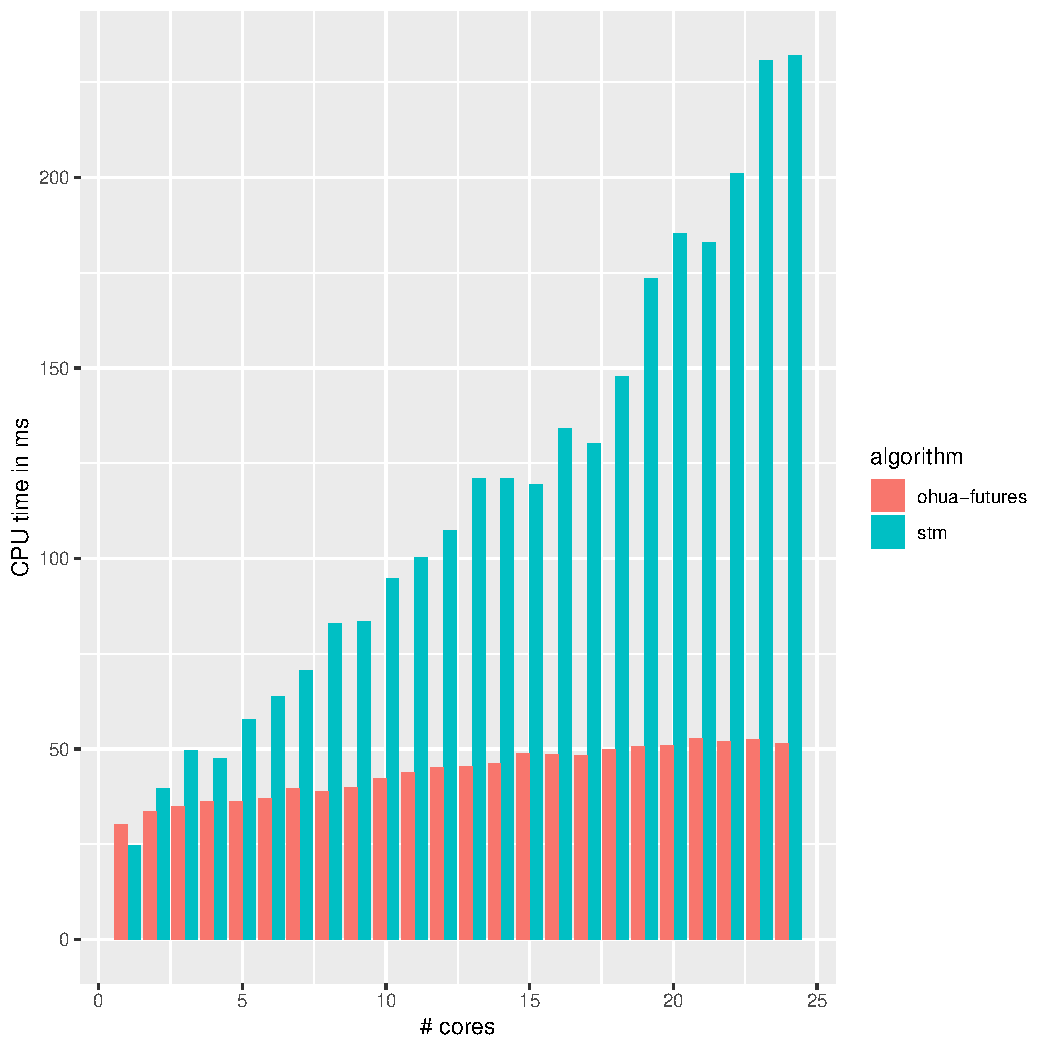
\includegraphics[width=\textwidth,keepaspectratio]{gfx/results/kmeans/kmeans-low_cpu}
        \caption{cpu usage kmeans-low}%
    \end{subfigure}%
    ~
    \begin{subfigure}[t]{.32\textwidth}
        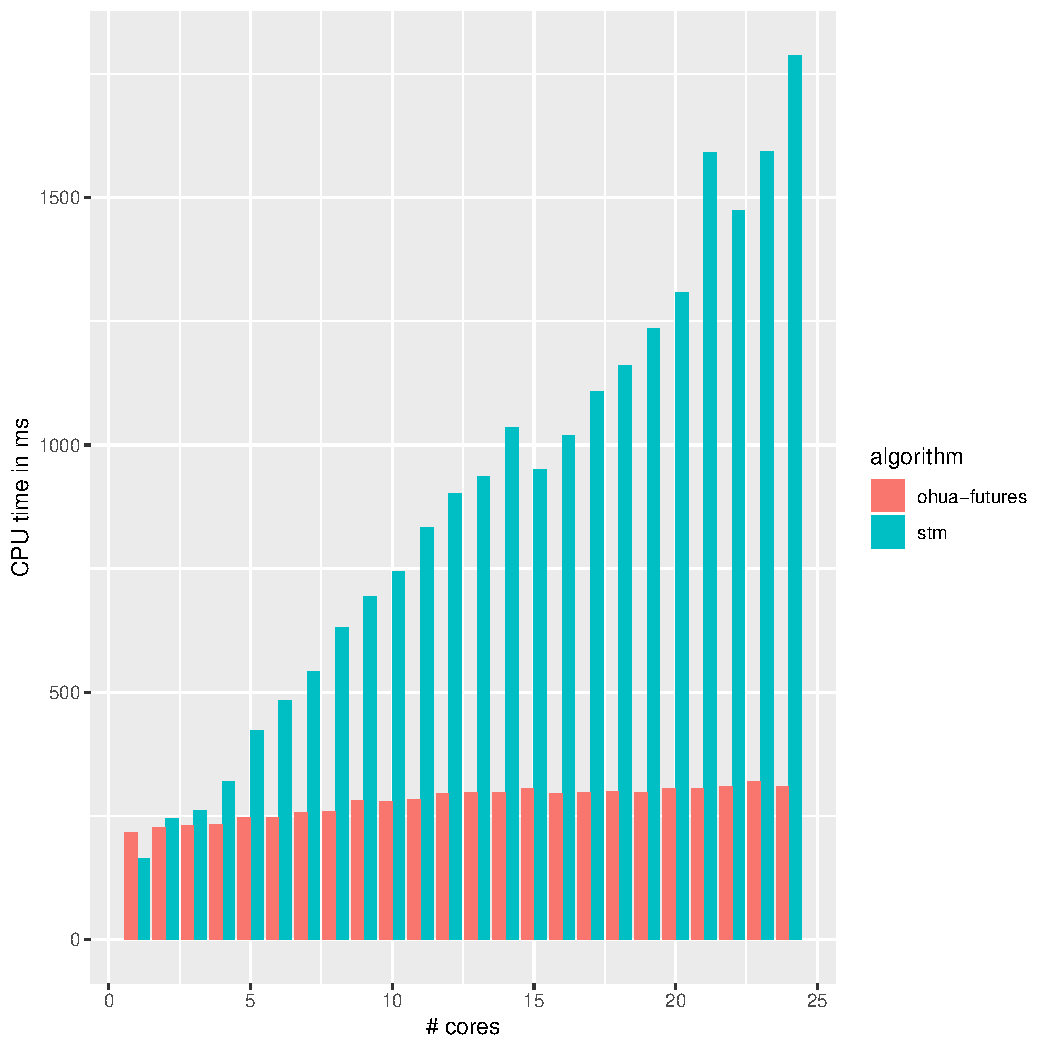
\includegraphics[width=\textwidth,keepaspectratio]{gfx/results/kmeans/kmeans-low+_cpu}
        \caption{cpu usage kmeans-low+}%
    \end{subfigure}%
    ~
    \begin{subfigure}[t]{.32\textwidth}
        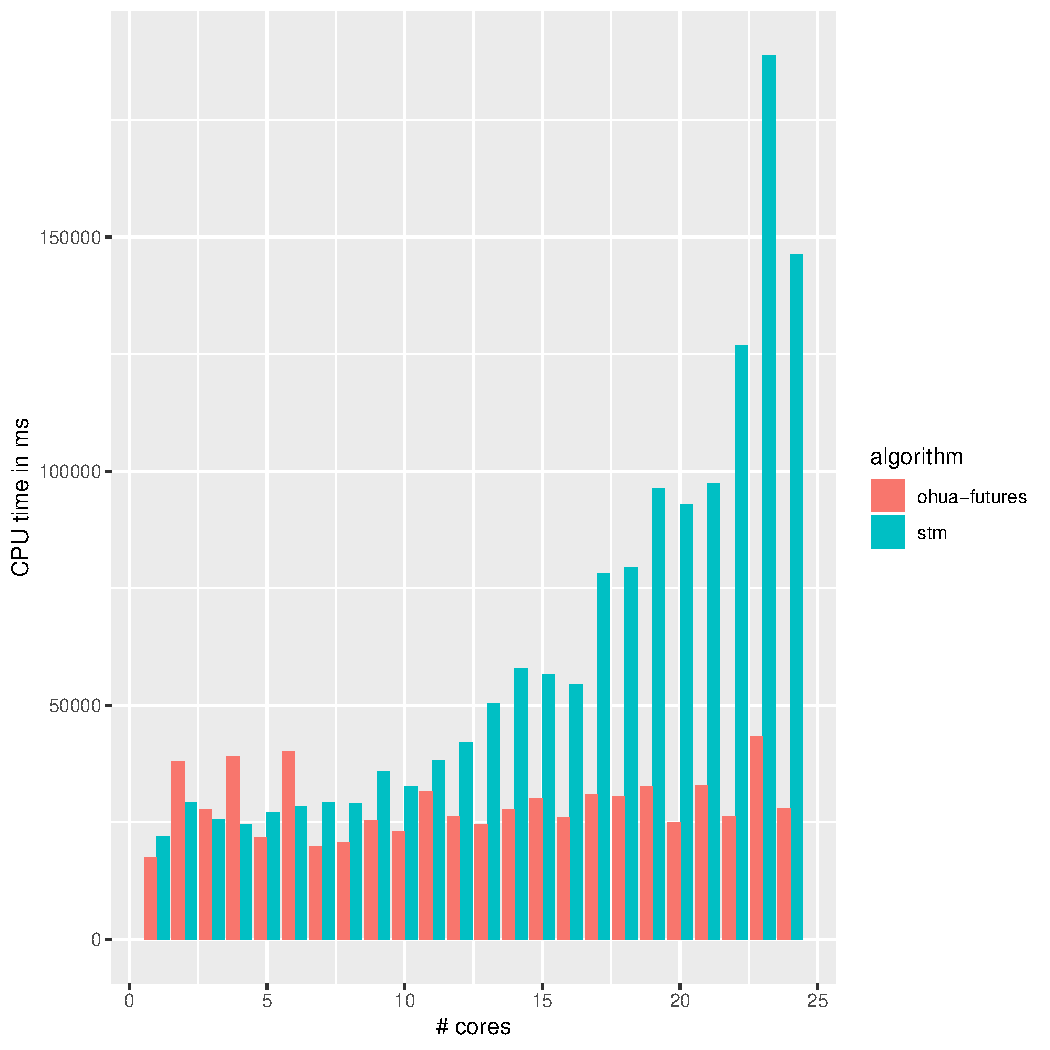
\includegraphics[width=\textwidth,keepaspectratio]{gfx/results/kmeans/kmeans-low++_cpu}
        \caption{cpu usage kmeans-low++}%
    \end{subfigure}%
    \caption{Results of the kmeans-low benchmark.}%
    \label{fig:evaulation:kmeans-low}
\end{figure}

% - present benchmark results -- maybe for the manual Ohua implementation as well, if results differ
% - discuss why we perform better/worse at certain points
% - we see the determinism!
% - discuss energy usage etc
